\chapter{Introduction}
\section{Motivation and goals}
Data compression plays a key role in hazard environments where computing power and data links are very limited. Two examples of these environments are outer space and undersea. In addition, some technologies used to capture data are proprietary and the data structure is not optimal for general purpose compressors such as GZIP.

This thesis is part of two strategic projects of Dapcom Data Services: the first one intended to compress \acrfull{rf} data, mainly from \acrshort{sdr} devices; and the second one focused on compressing the water column information contained in the KMALL format, a new data structure from Kongsberg Maritime.

Our goals are quite simple: we aim to develop two stages which perform better, in terms of compression ratio and speed, than already existing algorithms. Specifically, we will compare the first stage with \acrshort{flac}, a well-known audio encoder, and GZIP. The second stage will be only compared with GZIP, we haven't been able to find any more specific compressors for such format. Additionally, we also want to propose a universal metric to quantify the performance of new stages in terms of information.

\section{Thesis outline and organization}
This thesis starts in chapter \ref{ch:entropy_coding} with a theoretical approach to Information Theory. There, we describe some basic concepts which will be used later, for instance differential entropy or Golomb coding.

In chapter \ref{ch:fapec} we describe the key aspects of the \acrshort{fapec} framework and the current features and stages. Then, in chapter \ref{ch:new_stages} we state the general requirements and specifications for new stages. In this chapter we also propose some metrics to evaluate preprocessing stages.

Next two chapters correspond to the two preprocessing stages we propose. The outline for both chapters \ref{ch:wave_preproc} and \ref{ch:kmall_preproc} is almost the same: first we introduce the data format, then we propose an algorithm and finally we evaluate it using the metrics from chapter \ref{ch:new_stages}.

The last chapter consists in concluding the thesis and describing some possible future lines to work with.

Finally, the LaTeX source code of this thesis and the Python scripts used to evaluate the stages can be found in the following GitHub repository: \url{https://github.com/aniolm9/bsc-thesis-fapec}.

\section{State of the art}


\section{Project planning and costs}
\subsection{Gantt diagram}
From the critical review to this final document there have been some changes to the planning. The most relevant is that we added a new work package to find a linear invariant metric to evaluate the stages proposed in this thesis. We also added a new work package for the oral presentation preparation.

The final Gantt for this project is the following:
\begin{figure}[h!]
	\begin{center}
		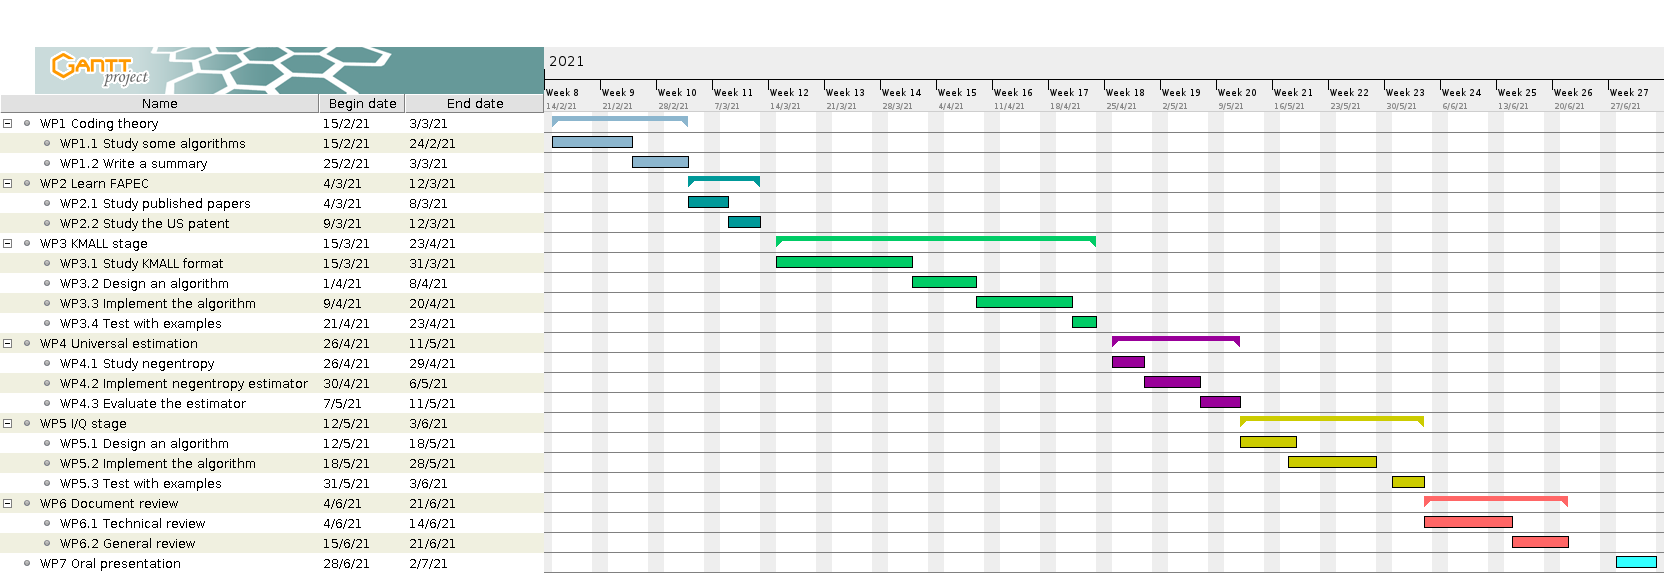
\includegraphics[scale=0.255]{images/gantt.png}
	\end{center}
	\caption{Final Gantt diagram.}
	\label{fig:gantt}
\end{figure}

\subsection{Budget and costs}
This thesis consists in the design, implementation and evaluation of two stages which will be included in a bigger framework, \acrshort{fapec}. In such situation, a financial study of only the stages is not possible, and studying the whole financial viability of \acrshort{fapec} is clearly out of the scope.

However, this thesis has been developed within a cooperation agreement between the Polytechnic University of Catalonia (UPC) and DAPCOM Data Services, with a cost of 3816€.
